\documentclass{article}
\usepackage{graphicx}
\usepackage{hyperref}
\usepackage{amsmath,amssymb}

\title{\textbf{Distributed and Concurrent Programming}\\ Second Assignment}

\author{
    \\Matteini Mattia
    \\Paganelli Alberto
}

\date{May 17, 2023}

\begin{document}

    \maketitle

    \begin{abstract}
        Il problema sottoposto è lo stesso di quello relativo al primo assignment.
        Nello specifico si richiede di leggere ricorsivamente dei file sorgenti (.java) partendo da una determinata cartella e categorizzandoli in base a quante linee hanno, rispettando i parametri inseriti dall'utente (approccio, intervalli, numero massimo di linee).
        In questo elaborato saranno sperimentati quattro approcci: il primo è un approccio a \texttt{Task} utilizzando il framework Executor di Java, il secondo sfrutta i \texttt{Virtual Threads}, il terzo utilizza il paradigma \texttt{Event Loop} tramite framework Vert.x, ed infine, come ultimo viene proposto un esempio di \texttt{Reactive Programming} grazie al framework RxJava.


    \end{abstract}


    \section{Architettura}
    L’elaborato si compone di due parti principali: la libreria adibita alla risoluzione del problema e un'applicazione client che la va ad utilizzare.
    Dalla libreria abbiamo deciso di esporre un'interfaccia \texttt{SourceAnalyzer} e un’istanza Singleton che la implementa, in modo tale da rendere immediato il suo utilizzo al client.
    \\
    L’interfaccia espone tre metodi:

    \begin{enumerate}
        \item \texttt{getReport()} che restituisce in maniera bloccante il risultato dell’analisi dei file restituendo una classe Report.
        \item \texttt{analyzeSources()} che restituisce in maniera incrementale il risultato, richiamando un handler ogniqualvolta viene processato un file.
        \item \texttt{stopAnalyzing()} che interrompe l’esecuzione del metodo \texttt{analyzeSources()}.
    \end{enumerate}

    La parte client si divide in un’applicazione con GUI e in una senza.
    Nel package senza interfaccia grafica si trovano le singole classi che utilizzano il metodo \texttt{getReport()}, una per ogni approccio.
    Nell'applicazione con GUI, strutturata con un minimale MVC, si può effettuare l’analisi dei file incrementale col metodo \texttt{analyzeSources()}, permettendo di scegliere l’approccio e interrompendolo se necessario.


    \section{Modellazione}


    \subsection*{Aggiornamento della grafica}

    L'aggiornamento della GUI viene fatto attraverso un handler passato nel metodo \texttt{analyzeSources()}, il quale viene richiamato ogni volta che un file viene processato.
    \\
    Nello specifico l'aggiornamento della grafica viene effettuato dall'Event Dispatcher Thread (EDT) utilizzando le \texttt{SwingUtilities}.
    \\
    Tuttavia in base all'approccio selezionato, il metodo di invocazione dell'EDT cambia, questo perché
    utilizzando l'approccio a Task o Virtual Threads, l'handler potrà essere chiamato da threads diversi, generando così problemi di concorrenza. In questo caso quindi si fa uso del metodo \texttt{invokeLater()} e di un Monitor.
    \\
    Utilizzando invece i paradigmi Event Loop e Reactive Programming, l'handler verrà innescato sempre e soltanto dal Thread del flusso di controllo principale, di conseguenza con il metodo \texttt{invokeAndWait()} non sarà mai necessario l'utilizzo di un Monitor dato che il flusso di controllo principale verrà messo in pausa durante l'aggiornamento della GUI.
    \\
    È stata presa questa decisione per mantenere la coerenza con i singoli paradigmi, evitando di introdurre problemi di concorrenza tramite l'utilizzo asincrono dell' EDT.
    \\


    \subsection{Approccio a Task}
    Adottando l’approccio orientato a \texttt{Task}, il sistema è stato modellato astraendo dai thread fisici sottostanti, ed è stata progettata una soluzione divisa in tasks dei quali non è necessario tenere conto di chi e come li esegue a basso livello.
    \\
    In questo caso sono state progettate due tasks: una relativa alla lettura massiva di file dalla directory ed una relativa alla lettura delle linee di un singolo file.
    Abbiamo fatto questa scelta per massimizzare l’indipendenza tra un task e l'altro e non avere strutture dati condivise.
    \\
    Tuttavia è inevitabile che si utilizzi un monitor nel momento in cui viene aggiornata la View attraverso l'handler fornito dal client.
    \\
    Mantenendo lo stesso procedimento adottato nel primo assignment, l’esecuzione del primo task è stata data in carico ad un Single Thread Executor (che svolge il task utilizzando un thread gestito e ottimizzato internamente).
    Una volta che l’executor ha terminato, per ogni file letto viene creato un task adibito al conteggio delle linee.
    \\
    Questi tasks sono sottoposti ad un Cached Thread Pool Executor che li esegue utilizzando un numero di thread non definito e che dipende dalla quantità di tasks sottoposti. La particolarità di questo executor è che appena un thread si libera dal suo compito viene subito riutilizzato (quando possibile) per eseguirne un altro, evitando di allocare altre risorse e rendendo così il Cached Thread Pool la scelta ottimale per soddisfare numerosi tasks di breve durata.


    \subsection{Approccio a Virtual Threads}
    In questo approccio sono stati utilizzati gli stessi tasks definiti nel precedente, e verranno mandati in esecuzione da un \texttt{VirtualThreadPerTaskExecutor}, il quale creerà un nuovo \texttt{Virtual Thread} per ogni task.
    \\
    La particolarità dei virtual threads è che ci permettono di astrarre dal concetto di thread tradizionale, consentendo di ignorare alcune limitazioni di questi ultimi come l’allocazione delle risorse.
    \\
    Infatti, le informazioni di contesto dei virtual threads vengono memorizzate nello Heap, a differenza dei threads tradizionali che invece risiedono nello Stack.
    Questo consente la creazione di tanti virtual thread quante sono le task senza incorrere in problemi di saturazione dello Stack.
    \\
    Quando un virtual thread entra in esecuzione, vengono recuperate le informazioni di contesto necessarie dallo Heap, vengono allocate nello Stack e deallocate non appena possibile (per lasciare spazio ad altri threads).
    \\
    Per quanto riguarda il monitor, sono state introdotte delle modifiche a causa dell’incompatibilità tra i blocchi \texttt{synchronized} e i virtual threads.
    Si è fatto uso di una variabile \texttt{Lock} e di una variabile \texttt{Condition}, così da ottenere lo stesso funzionamento atteso con i blocchi \texttt{synchronized}.



    \subsection{Approccio a Event Loop}
    In questo approccio si è fatto uso del Framework \texttt{Vert.x}.
    Dopo aver creato un’istanza di vertx, è stato fatto il deploy di un \texttt{Verticle} che incapsula il funzionamento di un \texttt{Event Loop}.
    \\
    Anche in questo caso il lavoro è stato suddiviso in due parti: la prima è inerente alla lettura dei file mentre la seconda al conteggio delle linee e gestione del risultato.
    \\
    La lettura dei file, a prescindere dal metodo chiamato dall’utente, è stata eseguita in maniera asincrona tramite l’utilizzo del metodo \texttt{executeBlocking()}. Una volta terminato verrà messo in coda un evento che gestirà il risultato (la lista di percorsi dei files).
    \\
    Viene usato lo stesso metodo asincrono anche per il conteggio delle linee dei singoli file, ma in base al metodo chiamato il risultato verrà gestito in maniera diversa.
    \\
    Se si chiama \texttt{getReport()}, prima di tornare il risultato si attende che tutte le \texttt{Futures} giungano al completamento con il metodo \texttt{CompositeFuture.all()}, e solo successivamente sarà possibile restituire il report.
    \\
    Se si chiama \texttt{analyzeSources()}, ogni volta che una \texttt{Future} viene completata, verrà chiamato l’handler di aggiornamento della View fornito dall’utente.


    \subsection{Approccio Reactive Programming}
    Per l’ultimo approccio è stato utilizzato il framework \texttt{RxJava}, che permette l’utilizzo del paradigma \texttt{Reactive Programming}.
    \\
    Anche in questo caso, a prescindere dal metodo chiamato dall’utente, per la lettura dei file viene creato un \texttt{cold stream} con un solo item all’interno (il percorso da analizzare). Questo stream viene mappato in uno contenente la serie di path di ogni singolo file da leggere.
    \\
    A questo punto si potrà accedere alla lista di path effettuando una \texttt{subscribe} allo stream.
    \\
    Successivamente, se si è chiamato \texttt{getReport()}, verrà generato un altro cold stream che mappa il Path ad un Pair contenente il nome del file e il numero di linee. Essendo cold, attraverso una subscribe si è sicuri di aver processato tutti i Path presenti nello stream e si potrà procedere alla creazione del report.
    \\
    Se invece si è chiamato \texttt{analyzeSources()}, verrà generato un \texttt{hot stream}, al quale viene fatto immediatamente subscribe per non perdere nessun file processato. Il funzionamento rimane lo stesso di \texttt{getReport()}, questa volta l’handler della subscribe verrà innescato ogni volta che viene processato un file, ovverosia ogni volta un elemento viene modificato nello stream attraverso la map.

    \clearpage
    \section{Risultati Computazionali}
    Il programma è stato testato selezionando in input una cartella con 2150 file sorgenti con numero di righe di codice variabili.
    \\
    È stato effettuato un test per ogni approccio e per ogni metodo. I test per \texttt{analyzeSources()} sono effettuati dall'applicazione con GUI, mentre quelli per \texttt{getReport()} sono effettuati da console.
    Di seguito sono mostrati i risultati dei test effettuati  esprimendo in media arrotondata il tempo impiegato:
    \footnote{I test sono stati effettuati senza l'utilizzo della cache. L'architettura utilizzata è ARM (Apple Silicon M1 Pro) con 10 core.}
    \begin{itemize}
        \item Approccio a Task GUI: $\Rightarrow 700 ms$
        \item Approccio a Task NO GUI: $\Rightarrow 700 ms$
        \item Approccio a Virtual Threads GUI: $\Rightarrow 1100 ms$
        \item Approccio a Virtual Threads NO GUI: $\Rightarrow 1100 ms$
        \item Approccio a Event Loop GUI: $\Rightarrow 1100 ms$
        \item Approccio a Event Loop NO GUI: $\Rightarrow 750 ms$
        \item Approccio a Reactive Programming GUI: $\Rightarrow 1300 ms$
        \item Approccio a Reactive Programming NO GUI: $\Rightarrow 1000 ms$
    \end{itemize}

    Si può notare che la differenza di tempo tra le versioni GUI e Console degli approcci a Task e a Virtual Thread è pressochè nulla. Questo perché l'aggiornamento della GUI viene effettuato in concorrenza dall'Event Dispatcher Thread.
    Al contrario per quanto riguardo i restanti due approcci, l'aggiornamento della GUI viene effettuato tramite il metodo \texttt{invokeAndWait()}, il quale esegue le modifiche alla GUI mettendo in pausa il principale flusso di controllo. Questo è necessario perché in questi due paradigmi, se non si vuole usufruire di un Monitor, il thread del flusso di controllo non può effettuare modifiche in concorrenza con l'Event Dispatcher Thread.


    \clearpage

    \section{GUI}
    \begin{figure}[h]
        \centering
        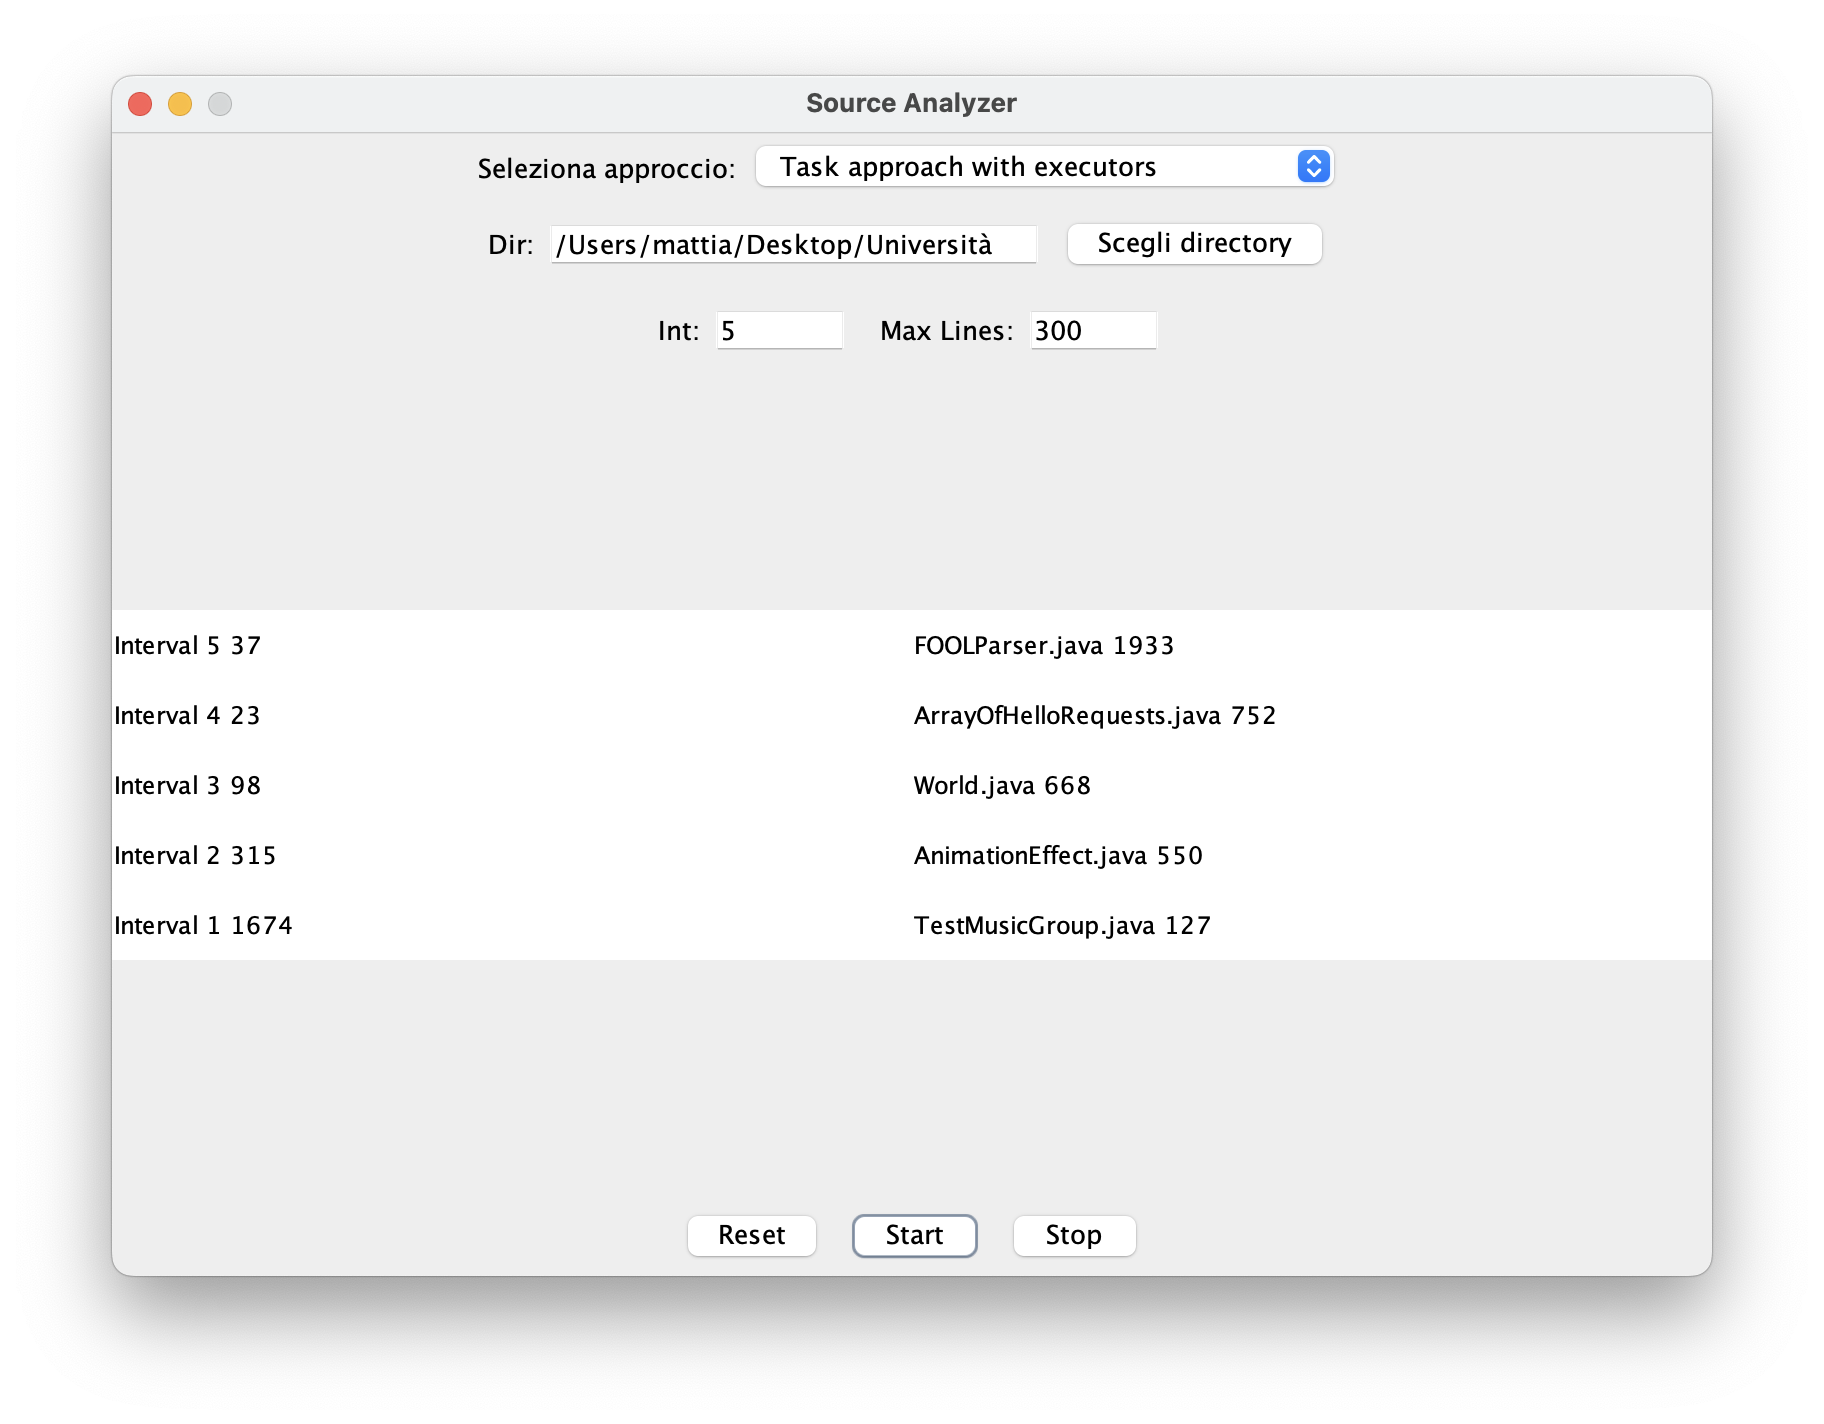
\includegraphics[width=1\linewidth]{screen-gui.png}
        \caption{Screen GUI}
        \label{fig:screen-gui}
    \end{figure}

\end{document}